\documentclass[11pt, letterpaper]{article}
\usepackage[backend=bibtex]{biblatex}
\bibliography{bib}
\usepackage[utf8]{inputenc}
\usepackage{amsmath}
\usepackage{amsfonts}
\usepackage{amssymb}
\usepackage{fullpage}
\usepackage{lmodern}
\usepackage{graphicx}
\usepackage{gensymb}
\usepackage{parskip}
\usepackage{tikz}
\usepackage{tikz-timing}
\author{Revan~Sopher}
\title{Detecting Planes in Real-Time for Camera Display Communications\\
{\large Independent Study Report}}
\begin{document}
\maketitle

\begin{abstract}
We implement a prototype Android system for extracting a message from a subtly intensity-encoded carrier image.
The system is novel in that it requires no camera calibration in color, time, nor space: it is tolerant of variation in ambient light, temporal synchronization, and observation angle. The system demonstrates high accuracy running on consumer hardware.
\end{abstract}

\section{Introduction}

\subsection{Visual MIMO}
The aim of the Visual MIMO project thus far has been to embed messages within images by varying the intensity of patches of the image, and to reliably extract these messages from pictures of the image displayed on a screen.

The existing software system is capable of detecting the computer monitor, in order to to consider only the displayed image, but encounters difficulties with the variance in photometry dependent on camera and display type, and the spatial positioning of the two.
This is addressed via radiometric calibration: nearly invisible patches are created on the corners of the image using histogram equalization, creating calibration data.

Although the Visual MIMO project is intended to make use of the ubiquity of handheld cameras, previous work has been reliant on a precise, static configuration of high quality SLR camera and a desktop computer, with processing performed post hoc.

The purpose of this independent study independent study is to implement this algorithm on a mobile device.

\subsection{Mobile Challenges}

This requires special considerations and optimizations to compensate for the significantly weaker processor and average cameras: the processing limitations can be mitigated by lower level programming and memory management using the Android Native Development Kit, but the lower quality image and light sensors has no obvious fix.

The primary focus of this study is in addressing the issues that arise from the spatial differences between the camera and the screen: although radiometric calibration can mitigate such differences, the resulting calibration is only valid for the current position, resulting in a fragile setup unsuitable for casual demonstrations.

The goal is to increase the accuracy of imperfect positioning, without requiring explicit calibration.

\section{Message Encoding}
The source message is generated in MATLAB. The bit string message to be encoded is turned into an 8x10 grid where each sector is either ``on'' with an intensity of $\alpha$, or ``off'' with an intensity of $0$.
Higher values of $\alpha$ are more accurate, but more visible.
The edges of the blocks are blended to reduce the visual impact of the sharp edges.

This grid is added and subtracted to the carrier image to create two frames (Figure~\ref{fig:message}). These frames are displayed alternating on the computer screen.

\begin{figure}[hbtp]
\centering
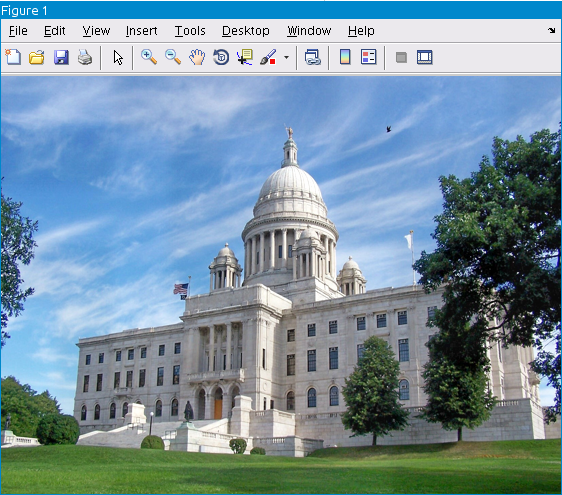
\includegraphics[scale=0.5]{img/message1.png}
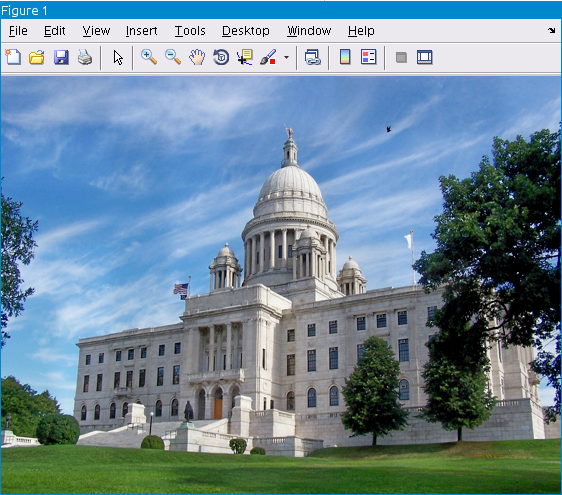
\includegraphics[scale=0.5]{img/message2.png}
\caption{An example of message embedding: the message is turned into a subtle grid pattern, then added and subtracted to carrier image to produce two frames.}
\label{fig:message}
\end{figure}

\section{Mobile Image Processing}

\subsection{Plane Tracking with Vuforia}
The Android application uses the Qualcomm Vuforia SDK \cite{vuforia}, a library meant for facilitating the construction of Augmented Reality applications.
Vuforia is used for its image tracking capabilities: known image targets are trained ahead of time, and are quickly and reliably detected in real-time.

Upon detection,	Vuforia provides the pose matrix. Combined with the known size of the target image camera parameters, we can calculate the position of the image corners, allowing us to process only the relevant part of the image.


\subsection{Skew Correction}
The usage of a mobile device for image capture necessarily forecloses angular calibration.
As such, the image captured is usually not perfectly head on.
In this step, we use a projective transformation to correct for skew.

First we obtain the $3 \times 3$ transformation matrix, such that:

$$
\begin{pmatrix}
t_i x_i^*\\
t_i y_i^*\\
t_i
\end{pmatrix}\\
= \text{transformation\_matrix} \cdot
\begin{pmatrix}
t_i x_i\\
t_i y_i\\
1
\end{pmatrix}
$$
That is, we map each corner to the proper rectangular positions.

Having calculated the corner positions previously and knowing the shape of the original image, this is easily accomplished with OpenCV\cite{opencv_getperspectivetransform}.

Next, we apply the transformation by multiplying the found matrix with each point in the image.
This is again straightforward with OpenCV \cite{opencv_warpperspective}, yielding Figure~\ref{fig:skew}.

\begin{figure}[hbtp]
\centering
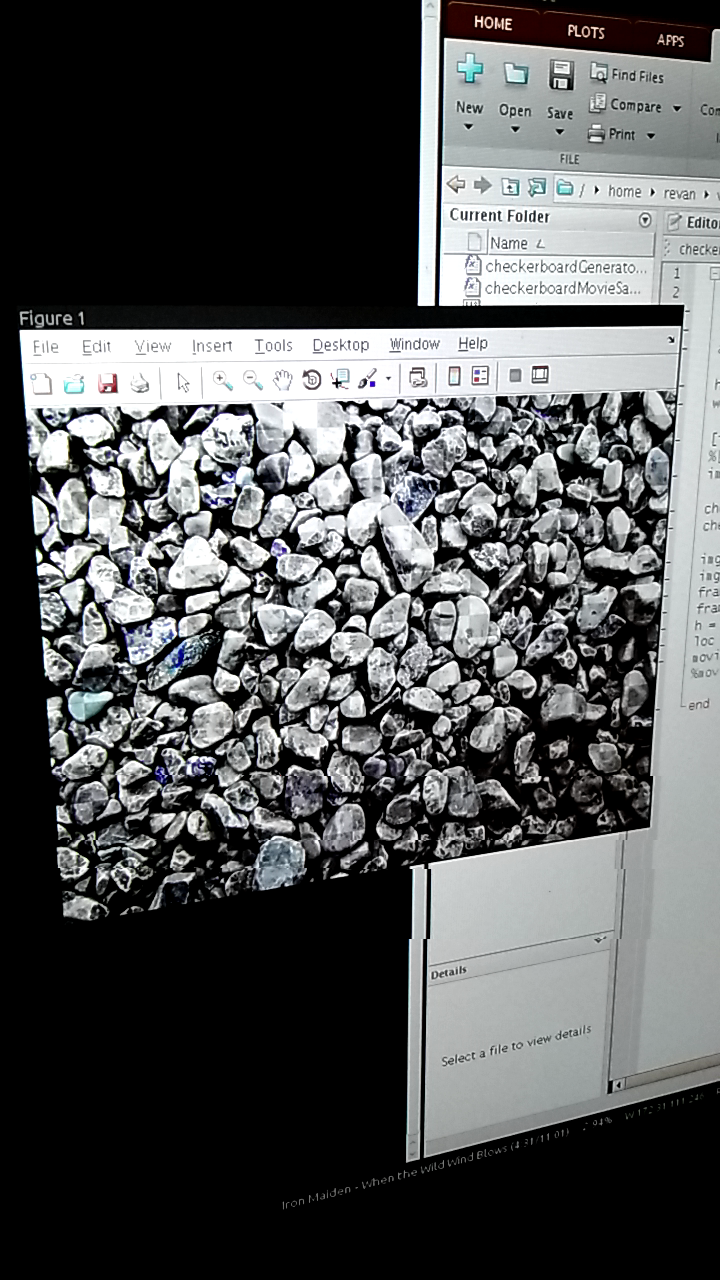
\includegraphics[scale=0.10]{img/skew.png}
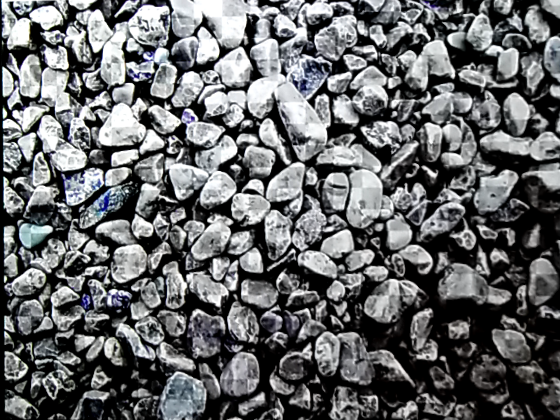
\includegraphics[scale=0.2]{img/skew2.png}
\caption{An image viewed at an oblique angle, then the image, skew-corrected and extracted by projective transformation.}
\label{fig:skew}
\end{figure}


\subsection{Histogram Equalization}
In the histogram equalization step, we improve the image contrast and transfer faithfulness by ``stretching'' the pixel intensity histogram to resemble a normal distribution (Figure~\ref{fig:histogram}).

We perform histogram equalization on both the source image and the captured image, which improves TODO CITATION.

Optimally we apply the same transformation to both images, however this is not especially straightforward using OpenCV so we rely on the two images having similar transforms and run the histogram equalization function twice.

\begin{figure}[hbtp]
\centering
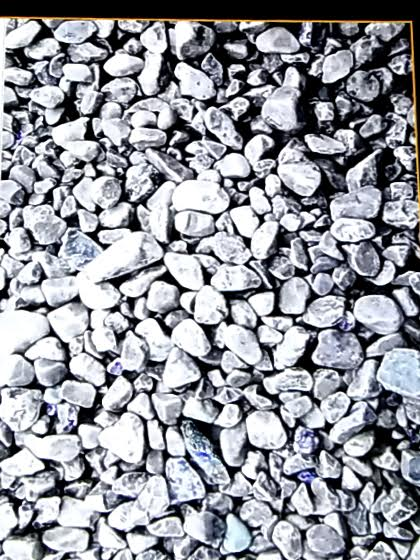
\includegraphics[scale=0.3]{img/histeq1.jpg}
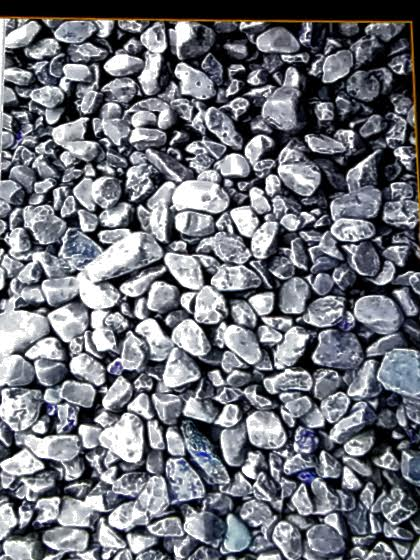
\includegraphics[scale=0.3]{img/histeq2.jpg}
\caption{An example of histogram equalization of an image: original on the left.}
\label{fig:histogram}
\end{figure}

\subsection{Subtraction}
With both targets skew-adjusted and normalized, we subtract one image from the other:

$$\text{dst}[I] = \text{saturate}(\text{src1}[I] - \text{src2}[I])$$ where $I$ is the image matrix\cite{opencv_subtraction}.

As the non-message part of the images should match up, this should leave only the message (Figure~\ref{fig:subtract}).

$$\frac{(\text{frame + message}) - (\text{frame - message})}{2} = \text{message}$$

\begin{figure}[hbtp]
\centering
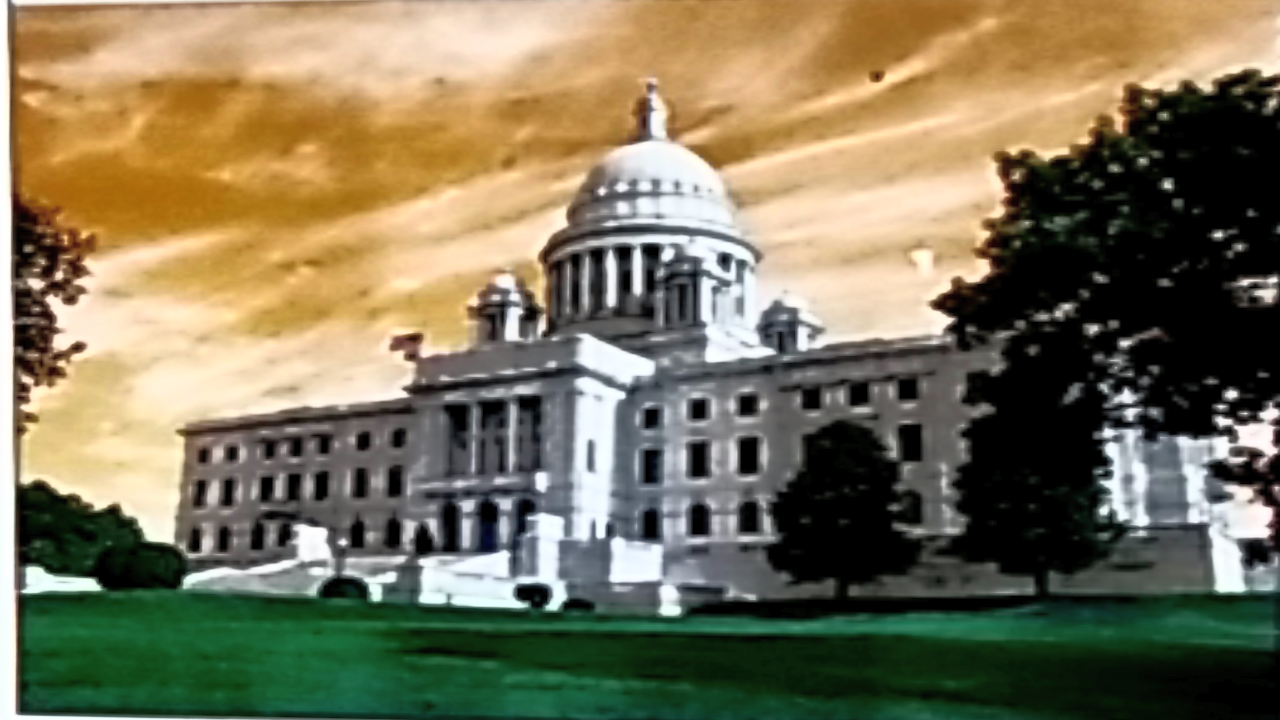
\includegraphics[scale=0.2]{img/subtract1.png}
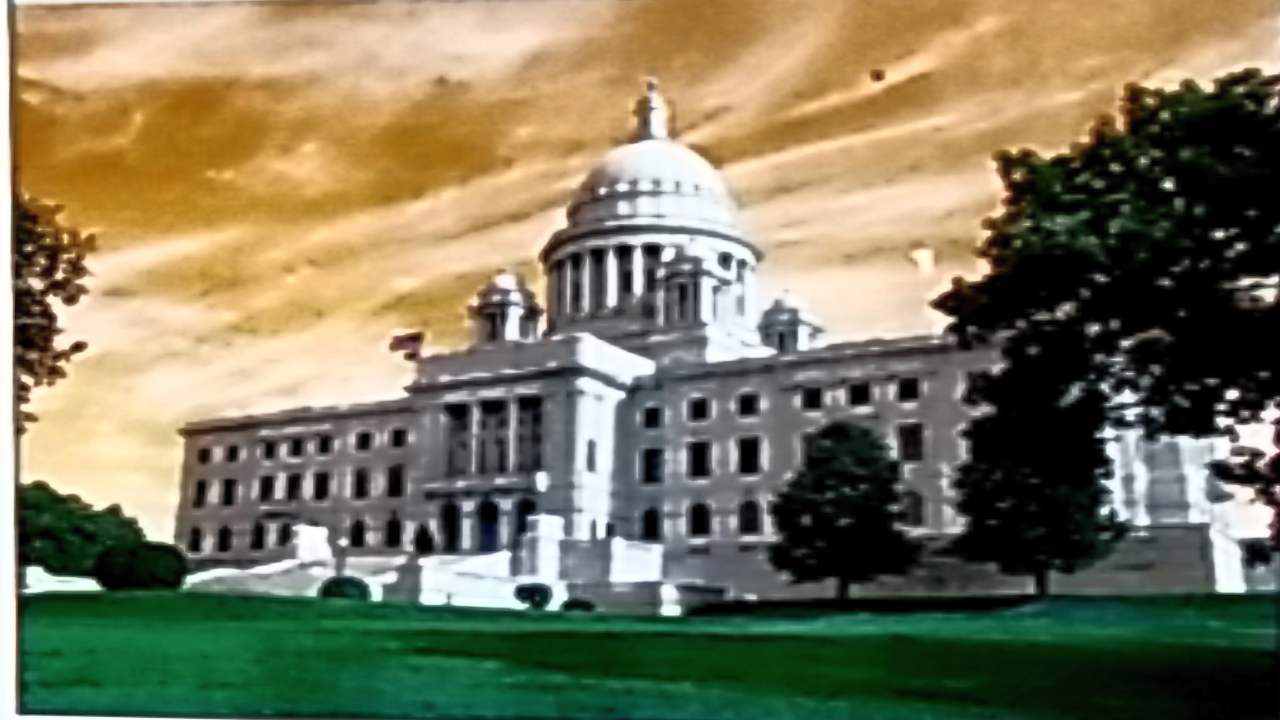
\includegraphics[scale=0.2]{img/subtract2.png}
\\
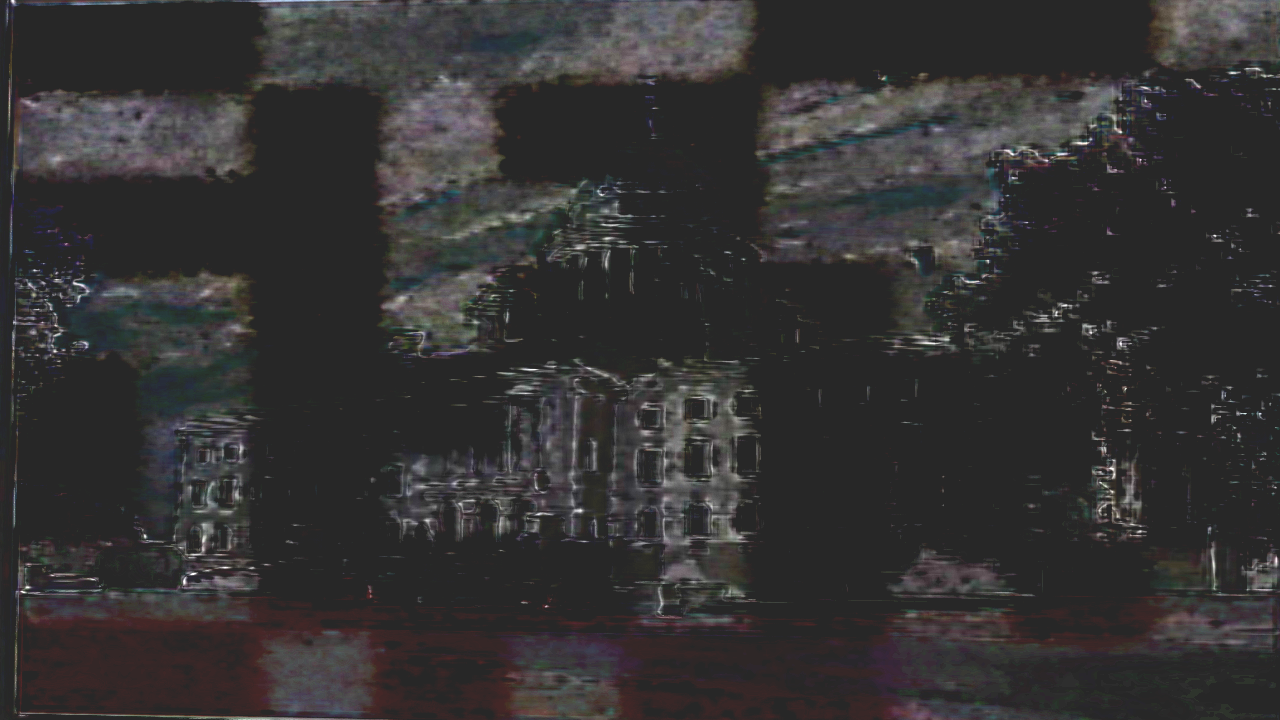
\includegraphics[scale=0.2]{img/subtract3.png}
\caption{An example of subtraction at $\alpha = 10$. 96.25\% accuracy on the retrieval of the embedded message "abcdefghijk".}
\label{fig:subtract}
\end{figure}

\subsection{Information Extraction}
Having isolated the encoded pattern, we must then decode the information inside.

We divide the difference image into a grid, and compare the average intensity of each sector against the average intensity of the entire image.
Assuming a mostly even distribution of 1's and 0's, the average intensity of the entire image will be approximately halfway between the ``on'' and ``off'' intensities. Thus we interpret any sector as a 1 or 0 depending on if its average intensity is greater or less than the general average.

We assemble the bit string, row by row.

\section{Synchronization}
Earlier iterations of the system had no synchronization measures in place, so the two frames chosen for subtraction were often not properly matched.
Combination such as both frames displaying the message added, or both subtracted, lead to nearly resulting images.

The system would also break when encountering frames that are between clean updates on the screen: there is a switching period involved in updating the source display.

\subsection{Multisampling}
This synchronization method involved taking four frames rather than just two, and selecting the best two frames to perform the subtraction and extraction on.
For each frame, we calculate the average intensity, and select the combination of two frames which maximizes the absolute value of the difference of their intensities.

We estimate that the refresh speed of the camera is ~20 FPS, so we fix the refresh speed of the encoded message at 10 FPS, the Nyquist frequency for this camera.

The reasoning for this method is based on the idea that the transitions between frames on the display are non-instantaneous, causing inaccuracies in decoding.
By sampling at twice the rate of the display, we can be reasonably sure that we will capture at least one clean picture of both frames, (img+msg) and (img-msg). (Figure~\ref{fig:multisampling}).

\begin{figure}[hbtp]
  \centering

  \Large

\begin{tikztimingtable}
  continuous displayed frames ($\frac{N}{2}$ Hz) & D 2m 6D{img+msg}  2m 6D{img-msg} 2m 6D{img+msg} 2m D\\
  4 camera samples ($N$ Hz) & 6s | 2{x 3D{clean} x 3D{dirty}} | \\
  \extracode
  \begin{pgfonlayer}{background}
  \begin{scope}[gray]
  \foreach \x in {3, 6, 6.5, 9.5, 10, 13, 13.5, 16.5}
  	\draw (\x, 0) -- (\x, -2);
  	\end{scope}
  	\end{pgfonlayer}
\end{tikztimingtable}

  \caption{Multisampling technique compensates for synchronization and switching times to reliably provide a clean image of both the positive and negative frames}
  \label{fig:multisampling}
\end{figure}

\section{Results}
TODO: data tables

\subsection{Various Carrier Images}

\subsection{Various $\alpha$ Values}

\subsection{Various Viewing Angles}

\section{Future Work}

\subsection{Multi-frame Messages}
The implementation described thus far only allows for as much information as can be encoded into a single image.
In order to scale this prototype arbitrarily, we must be able to encode and decode a series of messages sequentially.

To this end, the last few blocks of the message will be reserved for an index giving the position of the message relative to the other messages, in a Sliding Window implementation.
In such an implementation, the source display would loop through the series of messages, displaying the (img+msg) and (img-msg) of each frames once each.
The mobile device would begin collecting frames from an undefined point, using the encoded index to restructure the original message.

Synchronization in this design becomes problematic, however, as we must beware of attempting to difference mismatched frames.

\subsection{Google Glass}
Porting to Google Glass poses several problems. Primarily, the processing capabilities are limited: not only is the processor weaker, but the heat generated by performing heavy computations locally causes the device to overheat.
Therefore, the ``proper'' approach to such an application on Google Glass would consist of offloading all processing to a server, however this means such an implementation is less technically interesting.

\printbibliography
\end{document}
